\section{Strategie di distribuzione}
In questa sezione vengono esposte le scelte progettuali di distribuzione.

\subsection{Due possibili strategie di distribuzione}
\label{scelted}
Nella simulazione del traffico di una città, la politica di distribuzione che 
potrebbe ragionevolmente portare più benefici consiste nella segmentazione 
della dimensione della città. Questa politica, infatti, permette la distribuzione
su nodi diversi della simulazione dell'intera città. 
Seguendo questo approccio la città risulterebbe partizionata in quartieri, i
quali rappresenterebbero i frammenti dell'intera mappa della città, suddividendo
così su più nodi il luogo della realizzazione dello spostamento delle entità. 

Un'altra possibile strategia potrebbe essere quella di conservare in un unico
luogo la mappa, centralizzando su un singolo nodo lo stato di avanzamento del
sistema. Questa strategia non gode tuttavia della proprietà della scalabilità
della mappa: come si comporterebbe il sistema nel caso cambiasse la
configurazione della mappa e le dimensioni fossero notevoli? 
D'altro canto, questa strategia semplificherebbe di molto
la gestione dell'orologio virtuale per l'avanzamento delle entità del tipo veicolo,
bici o pedone dato che tutto, secondo la strategia in questione, diviene
centralizzato. Seguendo questa strategia la distribuzione potrebbe ricadere non
più sulla mappa ma sulle entità da spostare. Tuttavia il nodo che conserva
l'intera mappa diverrebbe un collo di bottiglia per gli aggiornamenti di stato
delle entità. 

\subsection{Strategia di distribuzione scelta}
La strategia scelta è la prima tra quelle esposte in \ref{scelted}. Questo
sistema risulta il più desiderabile in quanto sfrutta in modo adeguato il
concetto di distribuzione, permettendo così la gestione dei calcoli per
l'avanzamento delle entità e delle richieste su più nodi.

\subsection{Definizione dei ruoli delle entità del sistema}
Le entità esposte in \ref{firstmappa} meritano un ruolo in funzione della
strategia di distribuzione scelta. Fondamentalmente, le entità in un sistema
concorrente e distribuito vengono distinte in attive e reattive.
Assegnando il ruolo di entità attiva a veicoli, bici o pedoni si presenterebbe
un problema relativo al loro spostamento nel caso in cui essi debbano muoversi
da un quartiere all'altro.
Dato che le entità attive richiedono un processo, nel momento in cui un oggetto
debba spostarsi tra due quartieri, si incorrerebbe in un inutile spreco di
risorse, andando ad impattare anche le prestazioni del sistema.
Infatti, si avrebbe un processo inutile istanziato in un quartiere e
occorrerebbe istanziare uno di completamente nuovo nel quartiere di destinazione
dell'entità.
Questo potrebbe essere un problema dato che vengono istanziati dinamicamente dei
processi: si potrebbero ottenere errori a run-time nel caso in cui il nodo non
riesca ad istanziare il nuovo task.

L'alternativa potrebbe essere preallocare un certo numero di thread per ospitare
le entità che richiedono di essere spostate nel quartiere interessato.
A questo punto, però, occorrerebbe porre una limitazione sul numero di entità
che un certo quartiere potrebbe ospitare.
Questo risulterebbe quindi poco scalabile e scomodo da gestire nel caso in
cui un'entità attiva debba rimanere in attesa che il quartiere di
destinazione liberi un thread, dal proprio thread-pool di risorse preallocate,
per poterla eseguire.

Il ruolo di entità attiva dovrebbe ricadere quindi sugli oggetti di tipo strada
o incrocio. 
Dato che la mappa presenta, una volta configurata e istanziata, una un numero
costante di elementi, si avrà che il sistema non necessiterà di istenziare
dinamicamente dei processi.
Inoltre, ogni partizione per soddisfare le richieste di altre partizioni se
dotata di un thread-pool risolve anche il problema dell'allocazione di thread
per richieste remote da soddisfare.

Seguendo questa strategia il sistema diviene scalabile sia in termini di
distribuzione che di concorrenza.

\subsection{Componenti oggetto della distribuzione}\label{subsec:distribuzione}
\begin{figure}[H] % Example image
\center{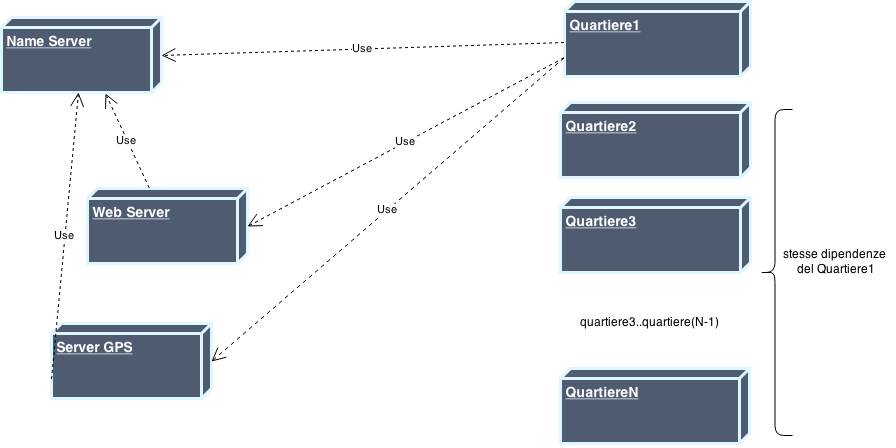
\includegraphics[width=1.0\linewidth]{DiagrammaComponenti}}
\caption{Diagramma componenti.}
\label{fig:Diagramma componenti}
\end{figure}
In questa sezione vengono descritte le componenti del sistema:
\begin{description}
\item[Quartiere:] componente che deve essere istanziata per ogni frammento della
mappa previsto dalla configurazione. Se un quartiere presenta una configurazione
valida, esso può entrare a far parte del sistema in qualunque momento (entro il
limite previsto del numero massimo di quartieri istanziabili).
Un quartiere è responsabile dello spostamento delle entità che sono in transito
in una qualunque delle strade o incroci che appartengono al quartiere stesso. Le
entità reattive quali i veicoli, le bici e i pedoni vengono istanziate in uno
specifico quartiere e le informazioni relative allo stato del percorso di queste
entità saranno sempre reperibili dal quartiere al quale l'entità è stata
istanziata, al fine di evitare che nel momento in cui un'entità debba essere
spostata da un quartiere all'altro, non occorra riportare tutto lo stato del
percorso al quartiere interessato.

Dato che, una volta configurato il sistema, le entità reattive non cambiano in
numero e contenuto informativo, conviene riportare per ogni quartiere una cache
delle entità di ogni altro quartiere al fine di evitare un numero eccessivo di
richieste a quartieri remoti responsabili dell'istanziazione delle entità
interessate durante le fase di avanzamento delle entità.
\item[Server GPS:] è una componente passiva che si occupa del calcolo del
percorso per conto di una entità. Questa componente dispone della conoscenza
della mappa di ogni quartiere correttamente istanziato. Il server GPS effettua
un aggiornamento della mappa in relazione alle nuove richieste di istanziazione
di nuovi quartieri. Il calcolo del percorso avviene eseguendo l'algoritmo di
Dijkstra dei cammini minimi. Se una certa entità deve muoversi verso una certa
destinazione non ancora raggiungibile, a causa del fatto che il quartiere
interessato non è stato ancora istanziato occorrerà ritardare lo spostamento
dell'entità. Il server per una stessa entità potrebbe calcolare percorsi minimi
diversi per 2 richieste diverse nel caso in cui nel frattempo è stato istanziato
un nuovo quartiere che presenta un percorso più breve per raggiungere la
destinazione.
\item[Web Server:] è la componente responsabile della creazione della view e
del rendering dello stato di avanzamento delle entità del sistema.
\item[Name Server:] si occupa invece di servire alle altre partizioni richieste
di accesso e riferimento a risorse che risiedono su una partizione remota.
\end{description}